\documentclass[twoside,11pt]{report}

% Any additional packages needed should be included after jmlr2e.
% Note that jmlr2e.sty includes epsfig, amssymb, natbib and graphicx,
% and defines many common macros, such as 'proof' and 'example'.
%
% It also sets the bibliographystyle to plainnat; for more information on
% natbib citation styles, see the natbib documentation, a copy of which
% is archived at http://www.jmlr.org/format/natbib.pdf

\usepackage{jmlr2e}
% \usepackage[utf8]{inputenc}%
% \usepackage{tikz}
% \usepackage{cfr-lm}%
\usepackage[T1]{fontenc}%
\usepackage{physics}
\usepackage{amsmath}
% \usepackage{amssymb}
% \usepackage{graphicx}
% \usepackage[margin=3cm]{geometry}
% \usepackage{changepage}
\usepackage{fontspec}
\usepackage{minted}
\usepackage{tcolorbox}
\usepackage{lmodern}
\usepackage{xcolor}
\usepackage{lettrine}
% \usepackage{fontawesome}
\usemintedstyle{perldoc}
\usepackage{hyperref}
\hypersetup{colorlinks=false, pdfborder={0 0 0},  }
\usepackage{fancyhdr}
\usepackage{wrapfig}
\usepackage{adjustbox}



\newtcbox{\codebox}[1][black]{on line, arc=2pt,colback=#1!10!white,colframe=white, before upper={\rule[-3pt]{0pt}{10pt}},boxrule=1pt, boxsep=0pt,left=2pt,right=2pt,top=1pt,bottom=.5pt}
\newtcbox{\deloppg}[1][black]{on line, arc=2pt,colback=#1!10!white,colframe=white, before upper={\rule[-2pt]{0pt}{0pt}},boxrule=0pt, boxsep=0pt,left=.49\linewidth,right=.49\linewidth,top=4pt,bottom=3pt}






% \setmainfont{FreeSans}
% \setmainfont{SF Pro Display}
% \setmainfont{IBM Plex Sans}
% \setmainfont{TeX Gyre Heros}
% \setmainfont{Inter}
% \setmainfont{Iosevka Quasi}

% \setmonofont{Iosevka Custom Extended}
% \setmonofont{JetBrainsMono Nerd Font}
% \setmonofont[Scale=MatchLowercase]{SF Mono}
\setmonofont[Scale=MatchLowercase]{IBM Plex Mono}






% Definitions of handy macros can go here

\newcommand{\dataset}{{\cal D}}
\newcommand{\fracpartial}[2]{\frac{\partial #1}{\partial  #2}}
\newtcolorbox[blend into=tables]{mytable}[2][]{float=htb, halign=center,  title={#2}, every float=\centering, #1 }
\newcommand\blfootnote[1]{ \begingroup \renewcommand\thefootnote{}\footnote{#1} \addtocounter{footnote}{-1} \endgroup }
% \definecolor{antwhite}{HTML}{323333}
\newcommand{\code}[3][]{\codebox{\mintinline[#1]{#2}{#3}}}
% Heading arguments are {volume}{year}{pages}{submitted}{published}{author-full-names}

% \jmlrheading{1}{2000}{1-48}{4/00}{10/00}{https://github.com/bragewiseth/MachineLearningProjects}

% Short headings should be running head and authors last names

\ShortHeadings{\url{https://github.com/bragewiseth/MachineLearningProjects}}{\url{https://github.com/bragewiseth/MachineLearningProjects}}
\firstpageno{1}



\title{{\huge Project 1}}
\author{\name Brage W. \email bragewi@ifi.uio.no\\
       \name Felix C. H.  \email felixch@ifi.uio.no \\
       \name Eirik B. J. \email eiribja@ifi.uio.no}
\date{\today}											% Date
\makeatletter






% \date{\today}

\begin{document}

%%%%%%%%%%%%%%%%%%%%%%%%%%%%%%%%%%%%%%%%%%%%%%%%%%%%%%%%%%%%%%%%%%%%%%%%%%%%%%%%%%%%%%%%%

\begin{titlepage}
	\centering
    \vspace*{0.5 cm}
    
\includegraphics[scale = 0.75]{uio.jpg}\\[1.0 cm]	% University Logo
    \textsc{\LARGE University of Oslo}\\[2.0 cm]	    % University Name
	\textsc{\Large FYS-STK3155}\\[0.5 cm]				% Course Code
	\rule{\linewidth}{0.2 mm} \\[0.4 cm]
	{ \huge \bfseries \@title}\\
	\rule{\linewidth}{0.2 mm} \\[1.5 cm]

	\begin{minipage}{0.4\textwidth}
		\begin{flushleft} \normalsize
            Brage Wiseth\\
            Felix Cameren Heyerdahl\\
            Eirik Bjørnson Jahr\\
			\end{flushleft}
			\end{minipage}~
			\begin{minipage}{0.4\textwidth}
			\begin{flushright} \normalsize
        \textsc{
          bragewi@ifi.uio.no\\
          felixch@ifi.uio.no\\
          eiribja@ifi.uio.no\\
        }
		\end{flushright}
        
	\end{minipage}\\[2 cm]
	\@date\\
    \vspace*{25mm}
    \urlstyle{rm}
    \textsc{\url{https://github.com/bragewiseth/MachineLearningProjects}}
	
	
    
    
    
    
	
\end{titlepage}
\nocite{*}
% \maketitle
\newpage
\tableofcontents
\newpage




\begin{abstract}%   <- trailing '%' for backward compatibility of .sty file
\lettrine{I}{}n this paper, we delve into the realm of machine learning model optimization and evaluation. 
Our study encompasses various regression techniques, including Ordinary Least Squares (OLS), Ridge, and 
Lasso regression, to analyze their effectiveness in handling simple and more complex datasets. Additionally, 
we employ bootstrap resampling and cross-validation methodologies to rigorously assess model performance 
and enhance generalization.
A significant portion of our investigation is dedicated to understanding the delicate balance between 
bias and variance. We explore how regularization methods like Ridge and Lasso impact bias-variance trade-offs, 
offering insights into the stability and predictive power of these models. Furthermore, we provide empirical 
evidence of the benefits of cross-validation and bootstrap techniques in mitigating overfitting and improving 
model robustness. We found that \{ ..results.. \}. Additionally we verify and compare our findings with well 
established theory and libraris such as SKLearn.
\end{abstract}
\begin{keywords}
    Linear Regression, Scaling, Bias \& Variance 
\end{keywords}









\section{Introduction}

Machine learning has emerged as a powerful tool in data analysis, providing the ability to uncover complex 
patterns and relationships in diverse datasets. But, at its core, machine learning is all about finding 
functions that capture the underlying structure of the data. The use of machine learning algorithms 
to approximate functions is the essence of this paper.\\

Our motivation for this research lies in the exploration of machine learning techniques to approximate 
the terrain on our planet, which can perhaps be described by such a function. Earth's terrain exhibits 
peaks and troughs, hills and valleys, much like some polynomial functions. Fortunately, we can employ 
standard linear regression techniques to approximate polynomials, but the terrain presents its own set 
of challenges. Firstly, the terrain's true underlying function may not be a polynomial at all, and its complexity may 
vary significantly from one location to another. Secondly, our landscape is teeming with small, intricate 
details. Some regions are characterized by flat and smooth surfaces, while others are marked by rough and 
uneven terrain. Focusing too much on these minute details can lead to model overfitting, making it crucial 
to strike a careful balance between model complexity and generalization.
In this context, regularization and resampling techniques, including Ridge and Lasso regression with bootstrap
and cross validation, have proven indispensable. By introducing regularization and resampling, we aim to find 
the sweet spot between bias and Variance. And getting the best predictions we can with our assumptions.\\
To embark on this exploration, we will begin with a simpler case: "Franke's function." which mimics our real terrain
data. This function 
serves as a foundational starting point, allowing us to assess our model's performance in a controlled 
environment before venturing into the complexity of real-world terrain data. Through this gradual progression, 
we provide ourselves wih a framework that can be applied to more complex and varied real-world terrain datasets.\\

\textbf{Data}: We begin by introducing the dataset used for our analysis, highlighting data collection and preprocessing procedures. 
Understanding the characteristics of the terrain data is fundamental to our modeling endeavor.\\
\textbf{Methods and Scaling}: Next, we delve into the methodology, encompassing the implementation of polynomial regression 
models and the application of regularization techniques such as Ridge and Lasso. Additionally, we will discuss the 
importance of proper scaling for model stability and convergence.\\
\textbf{Results}: In this section, we will present the outcomes of our experiments, showcasing the performance of different 
models and regularization techniques. Through empirical evidence, we aim to provide insights into the effectiveness of our approach.\\
\textbf{Bias-Variance Trade-off}: A significant portion of our study will revolve around the critical concept of bias and 
variance. We'll explore how regularization methods influence this trade-off and delve into the fine balance between 
model complexity and generalization.\\
\textbf{Conclusion}: Finally, we will summarize the key findings and their implications for terrain modeling with machine learning. 
Our conclusion will underscore the importance of regularization in achieving accurate representations of complex terrains and 
provide a perspective on future research directions.

\begin{center}
    \scriptsize code for generating all figures and data can be found at 
\href{https://github.com/bragewiseth/MachineLearningProjects/tree/main/project1/src}{\tt \textsc{/MachineLearningProjects/project1/src} }
\end{center}








\section{Data}
\label{sec:data}

The data we will be using consists of 100 points generated using the Franke function. The Franke function is a weighted sum of four exponentials given by
\begin{align*}
    f(x,y) &= \frac{3}{4}\exp\left(-\frac{(9x-2)^2}{4}-\frac{(9y-2)^2}{4}\right)\\
    &+ \frac{3}{4}\exp\left(-\frac{(9x+1)^2}{49}-\frac{(9y+1)}{10}\right)\\
    &+ \frac{1}{2}\exp\left(-\frac{(9x-7)^2}{4}-\frac{(9y-3)^2}{4}\right)\\
    &- \frac{1}{5}\exp\left(-(9x-4)^2-(9y-7)^2\right)
\end{align*}
Figure~\ref{fig:truefunction} shows a graphical representation of the Franke's function\\
We will add some noise to the data to better simulate real world data. 
\begin{figure}[!h]
\begin{minipage}[!t]{.48\linewidth}
    \begin{center}
        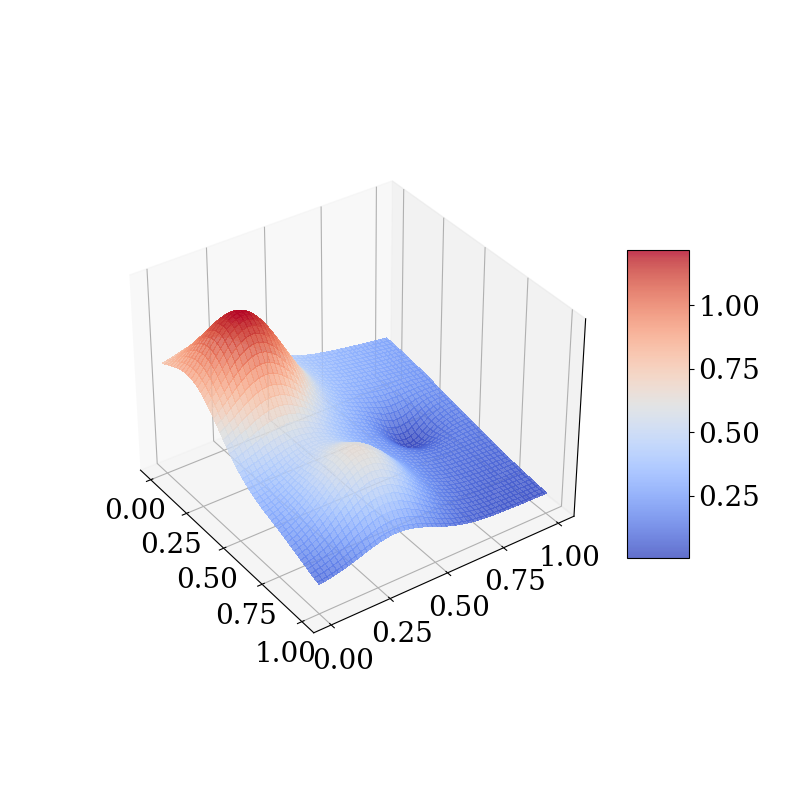
\includegraphics[width=1.1\textwidth]{../runsAndAdditions/trueFunction.png}
        \caption{True Function}\label{fig:truefunction}
\end{center}
\end{minipage}
\hspace{2mm}
\begin{minipage}[!t]{.48\linewidth}
    \begin{center}
        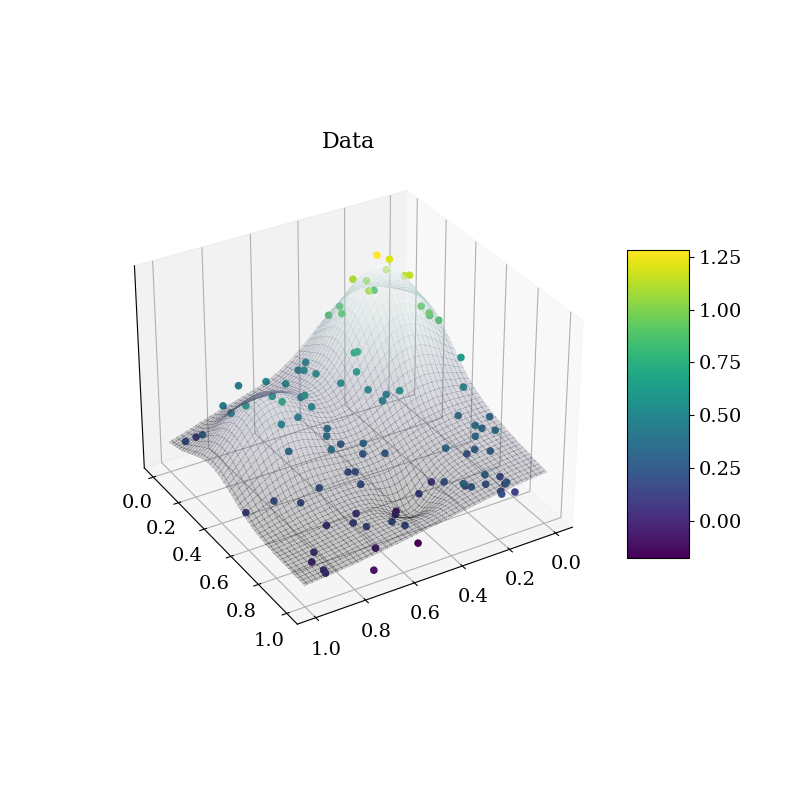
\includegraphics[width=1.1\textwidth]{../runsAndAdditions/synthDataSide.png}
        \caption{Our Synthetic Data}\label{fig:synthdataside}
    \end{center}
\end{minipage}
\end{figure}
\begin{figure}[!h]
\begin{minipage}[!t]{.48\linewidth}
    \begin{center}
        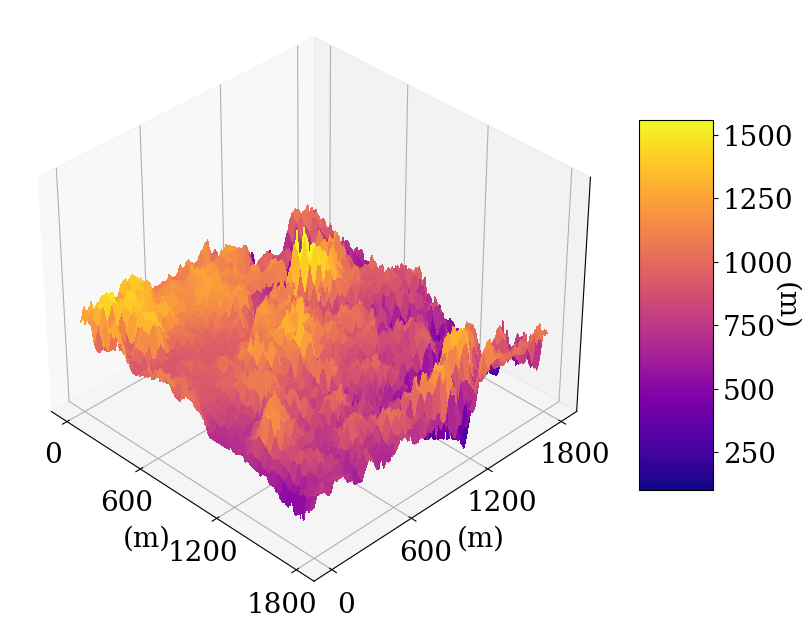
\includegraphics[width=1.0\textwidth]{../runsAndAdditions/realdata3D.png}
        \caption{True Function}\label{fig:realdata3D}
\end{center}
\end{minipage}
\hspace{2mm}
\begin{minipage}[!t]{.48\linewidth}
    \begin{center}
        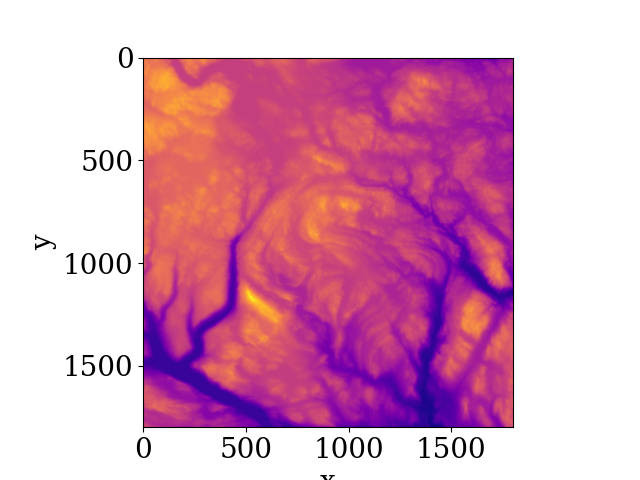
\includegraphics[width=1.0\textwidth]{../runsAndAdditions/realdataMap.png}
        \caption{Our Synthetic Data}\label{fig:realdataMap}
    \end{center}
\end{minipage}
\end{figure}
The noise is sampled from a normal distribution with mean 0 and variance $\sigma^2 = 1$.
The data is generated by sampling x and y from a uniform distribution on the interval $[0, 1]$.
In Figure~\ref{fig:synthdataside} you can see a representation of our data.
To apply our findings with this toy dataset to real-world data, we will also use a 
real topographic dataset from Norway see Figure~\ref{fig:realdata3D} and Figure~\ref{fig:realdataMap}. 
However, due to limited computational resources and the time it takes to run our program, we only sample 
40000 - 50000 points from about 3 million points. For both datasets we split the data is into 
training and testing sets, with the testing set comprising twenty percent. For some cases when running
resampling techniques we also split the data into training, validation and testing sets.

As we hinted at in the introduction, we will try to fit a polynomial to both datasets. That means that our input data will be 
the $x$ and $y$ values as well as higher order terms $x^2$, $y^2$, $xy$, $x^3$, $y^3$, $x^2y$, $xy^2$ and so on.
We have chosen to not include the first term of the polynomial, which is just $1$. This is because we will be scaling our data,
more on this in Section~\ref{sec:scaling}.\\








\section{linear regression models }
\label{sec:models}

Linear models assume that the relationship between the input variables (predictors or features) 
and the output variable (response or target) is linear. The predictions of the model is a linear
combination of the input variables with some coefficients. The coefficients are estimated from
the training data using a method called least squares. The least squares method is used to find
the coefficients that minimizes the residual sum of squares between the observed responses in
the dataset, and the responses predicted by the linear approximation. The residual sum of squares
is given by
$$
RSS(\beta) = \sum_{i=0}^{n-1} (y_i - \tilde{y}_i)^2
$$
where $y_i$ is the observed response for observation $i$, $\tilde{y}_i$ is the predicted response for observation $i$ 
$$
\bar{y} =  \frac{1}{n} \sum_{i=0}^{n - 1} y_i
$$
We can also take the mean of the residual sum of squares, which is called the mean squared error (MSE). This is what we will use to
evaluate our models. The MSE is given by
$$
\mbox{MSE}(\mathbf{y},\mathbf{\tilde{y}}) = \frac{1}{n}
\sum_{i=0}^{n-1}(y_i-\tilde{y}_i)^2
$$
We wil also use the $R^2$ score to evaluate our models. The $R^2$ score is a statistical measure of how close the data are to the fitted regression line. The $R^2$ score is given by
$$
R^2(\mathbf{y}, \tilde{\mathbf{y}}) = 1 - \frac{\sum_{i=0}^{n - 1} (y_i - \tilde{y}_i)^2}{\sum_{i=0}^{n - 1} (y_i - \bar{y})^2}
$$
The R2 score is a number between 0 and 1, where 1 indicates that the model fits the data perfectly. 
A negative R2 score indicates that the model is worse than just predicting the mean of the data.





\subsection{Ordinary Least Squares (OLS)}
\label{sec:ols}


By minimizing the MSE, we find the coefficients that minimizes the residual sum of squares. This is done by taking the derivative of the
MSE with respect to the coefficients $\beta_j$ and setting it equal to zero. This gives us the optimal parameters
$$
\hat{\boldsymbol{\beta}}_{\mathrm{OLS}} = \left(\mathbf{X}^T\mathbf{X}\right)^{-1}\mathbf{X}^T\mathbf{y}
$$
\begin{center}
    The derivation of this can be found in the appendix~\ref{app:OptimalBeta} 
\end{center}
The \emph{Design Matrix} $\mathbf{X}$ is a matrix of our input data, the columns of $\mathbf{X}$ are the features of our 
data and the rows are the observations. For our case the columns are the polynomial terms. \footnote{the first
term of a polynomial is just $1$, however we have chosen not to include this. more on this in Section~\footref{sec:scaling} 
about scaling}\\ 
We can then use these parameters to predict the response $\tilde{\mathbf{y}}$ for a new set of predictors $\mathbf{X}$.
The predictions is as previously mentioned a linear combination of the predictors and the coefficients.
$$
\tilde{\mathbf{y}} = \mathbf{X}\boldsymbol{\beta}
$$
Wich is a compact way of writing
$$
\tilde{y}_i = \beta_0 + \beta_1 x_{i1} + \beta_2 x_{i2} + \dots + \beta_{p-1} x_{i,p-1}
$$
where $p$ is the number of predictors.\\

\subsection{Ridge \& Lasso Regression}
\label{sec:ridge}

We can add add regularization to the linear regression model to help keep our parameters in check. 
This is done by adding a penalty term to the cost function. The penalty term is a function of the coefficients $\beta_j$. 
The penalty term is called the regularization term, and the parameter $\lambda$ is called the regularization parameter. 
The regularization parameter determines how much the coefficients are penalized. The cost function for Ridge regression is given by
$$
C(\mathbf{\beta}) = \frac{1}{n}\sum_{i=0}^{n-1}(y_i-\tilde{y}_i)^2 + \lambda\sum_{j=0}^{p-1}\beta_j^2  
=\frac{1}{n}\vert\vert \mathbf{y}-\mathbf{X}\mathbf{\beta}\vert\vert_2^2 + \lambda\vert\vert\mathbf{\beta}\vert\vert_2^2
$$




$$
\hat{\mathbf{\beta}}_{\mathrm{Ridge}} = \left(\mathbf{X}^T\mathbf{X}+\lambda\mathbf{I}\right)^{-1}\mathbf{X}^T\mathbf{y},
$$


Lasso regression is similar to Ridge regression, with the difference being that the penalty term is the sum of the absolute values of the coefficients $\beta_j$, also called 
the L1 norm. The cost function for Lasso regression is given by
$$
C(\mathbf{\beta}) = \frac{1}{n}\sum_{i=0}^{n-1}(y_i-\tilde{y}_i)^2 + \lambda\sum_{j=0}^{p-1}\vert\beta_j\vert
=\frac{1}{n}\vert\vert \mathbf{y}-\mathbf{X}\mathbf{\beta}\vert\vert_2^2 + \lambda\vert\vert\mathbf{\beta}\vert\vert_1
$$
We won't be utilizing our custom Lasso implementation and derivation; instead, 
we will opt for the Lasso implementation provided by the Scikit-Learn library.


\subsection{Scaling}
\label{sec:scaling}


\begin{mytable}[float=!h, label=tab:unscaled]{Unscaled design matrix fitting one-dimensional polynomial of degree 5}
\tt
\centering
\begin{tabular}{llllll}
    1. &     0.  &    0.  &    0.   &   0.   &   0.     \\
    1. &     0.25 &   0.0625 & 0.01562& 0.00391& 0.00098\\
    1.    &  0.5     &0.25 &   0.125 &  0.0625 & 0.03125\\
    1.   &   0.75  &  0.5625 & 0.42188 &0.31641& 0.2373 \\
    1.  &    1.   &   1.  &    1.  &    1.    &  1.
\end{tabular}%
\end{mytable}
\begin{mytable}[float=!h,label=tab:scaled]{Scaled design matrix fitting one-dimensional polynomial of degree 5}
\tt
\centering
\begin{tabular}{llllll}
     0. &     -1.41421& -1.0171&  -0.83189& -0.728 &  -0.66226\\
     0.  &    -0.70711& -0.84758& -0.7903 & -0.71772& -0.65971\\
     0.  &     0.    &  -0.33903& -0.49913& -0.56348& -0.58075\\
     0.  &     0.70711&  0.50855&  0.29116 & 0.10488& -0.0433 \\
     0.  &     1.41421&  1.69516 & 1.83016 & 1.90431&  1.94603
\end{tabular}%
\end{mytable}
\begin{mytable}[float=!h,label=tab:scaling]{MSE for scaled and unscaled data}
\centering
\begin{tabular}{ll}
mse for ols on unscaled data:    &   \texttt{0.010349396022903145} \\
mse for ols on scaled data:      &   \texttt{0.010349396024145656} \\
mse for ridge on unscaled data:  &   \texttt{0.02106077418650843} \\
mse for ridge on scaled data:    &   \texttt{0.01782525371566323}
\end{tabular}%
\end{mytable}
Consider Table~\ref{tab:unscaled}, Table~\ref{tab:scaled} and Table~\ref{tab:scaling}. At first glance, 
there isn't a big difference between the unscaled data and the scaled data. 
This is because the original data was already close to having a mean close to zero and not being spread out too much. 
So, you might think that scaling the data isn't necessary.
However, when we introduce polynomial terms, we notice that some values in xunscaled become extremely small. As an example, 
if we take $x=0.15$ and want to find some term $x^6$ that becomes roughly $0.00001$. This means that the columns of xunscaled have vastly different orders of magnitude, and this calls 
for scaling to bring them back to a similar scale.
If we don't scale, the coefficients $(\boldsymbol{\beta})$ can range widely, from $\pm 50$ in this example. 
But when we scale the data, this range narrows 
down to $\pm 10$. Now, this alone might not seem like a strong reason to scale the data, especially when we use plain 
linear regression (OLS), as it doesn't change the Mean Squared Error (MSE) much.\\
However, things change when we use Ridge regression. In Ridge, the regularization cost depends on the magnitude of $\beta_i$.
With unscaled data, where $\beta_i$ varies a lot, some coefficients get penalized more than others. This results in a 
significantly higher MSE for unscaled data compared to scaled data in Ridge regression.
So, to make it easier to tune the regularization parameter $(\lambda)$ and to ensure fair treatment of coefficients in Ridge regression, 
it's a good idea to scale the data. This not only simplifies the regularization process but also leads to better predictive performance.

Notice how the first column in Table~\ref{tab:scaled} becomes zero when we scale. This fact is what led us to exclude the first term of the polynomial.










\section{Results and Discussion}
\label{sec:resultsdiscussion}


For the relatively simple Franke's function, we must say that we are quite pleased with the results.
We have managed to fit a polynomial of degree 5 to the data with an $R^2$ score of $0.879$ and a MSE of $0.00855$ 
using OLS. Ridge yielded almost identical results  when using a small value of $\lambda = 10^{-6}$.
Lasso was lagging a bit behind with the best $R^2$ score of $0.852$ and a MSE of $0.0105$, 
also with a small value of $\lambda = 10^{-6}$.
\begin{mytable}[float=!h,label=tab:toyscores, width=0.5\textwidth]{Best scores from synthetic data}
\vspace{1mm}
\centering
\begin{tabular}{l|c|c|c}
    & OLS & Ridge & Lasso \\
    \hline
    MSE  &   \texttt{0.010349} & yurr & yurr \\
    $R^2$     &   \texttt{0.0103} & yurr & yurr \\
    $\lambda$ &  N/A  & $10^{-6}$ & $10^{-6}$ 
\end{tabular}%
\end{mytable}

\begin{figure}[!h]
    \begin{center}
        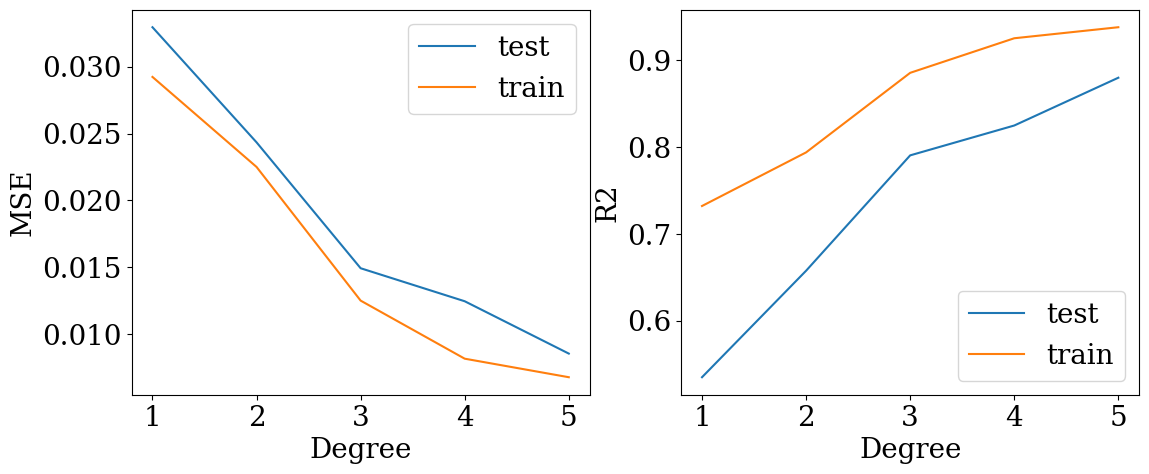
\includegraphics[width=0.95\textwidth]{../runsAndAdditions/R2andMSEOLS.png}
    \end{center}
    \caption{$R^2$ and MSE with increasing complexity}\label{fig:R2andMSEOLS}
\end{figure}

From Figure~\ref{fig:R2andMSEOLS} we can see that the MSE and $R^2$ both improve as we increase the model complexity, we have yet to see any signs of overfitting which indicates that we can increase the complexity even further.\\

\begin{minipage}[!t]{.48\linewidth}
    \begin{center}
        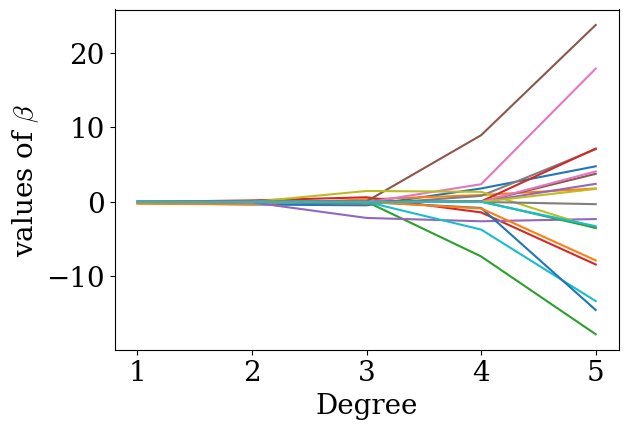
\includegraphics[width=1.0\textwidth]{../runsAndAdditions/betaOverOrderOLS.png}
\end{center}
\end{minipage}
\hspace{4mm}
\begin{minipage}[!t]{.48\linewidth}
    \begin{center}
        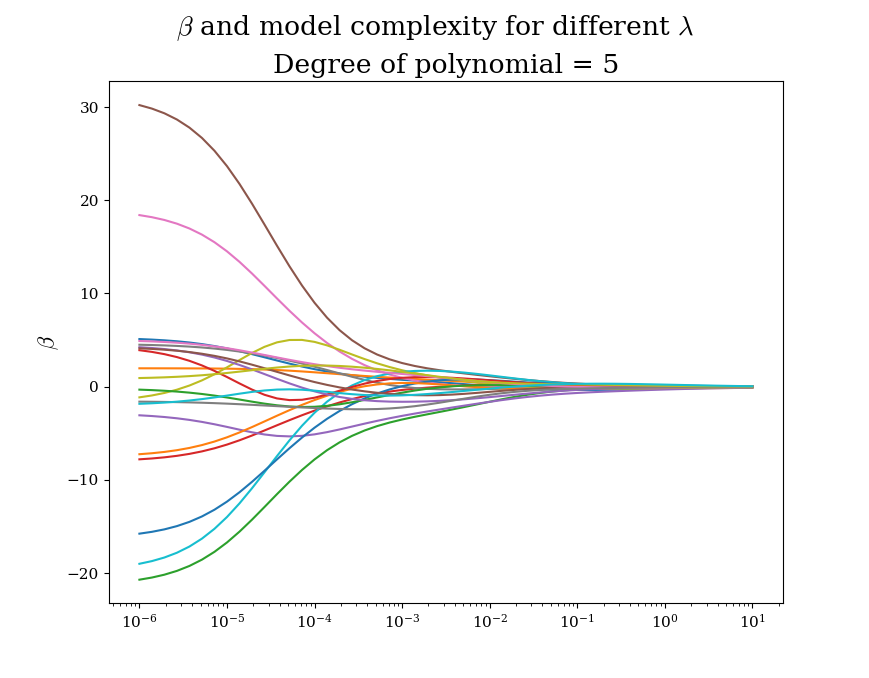
\includegraphics[width=1.0\textwidth]{../runsAndAdditions/BetaOverLambdaRidge5.png}
    \end{center}
\end{minipage}



\begin{minipage}[!t]{.48\linewidth}
    \begin{center}
        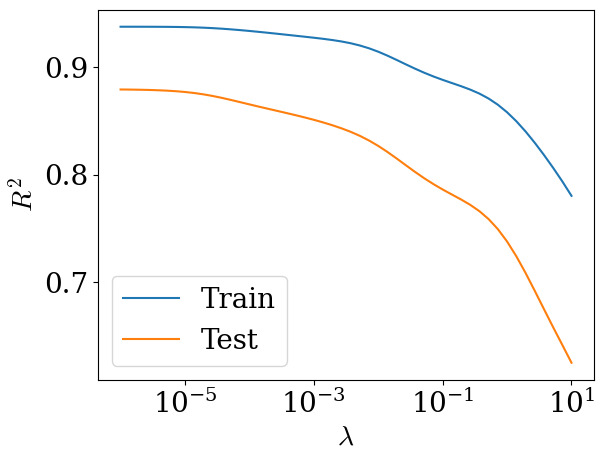
\includegraphics[width=1.0\textwidth]{../runsAndAdditions/R2OverLambdaRidge5.png}
\end{center}
\end{minipage}
\hspace{4mm}
\begin{minipage}[!t]{.48\linewidth}
    \begin{center}
        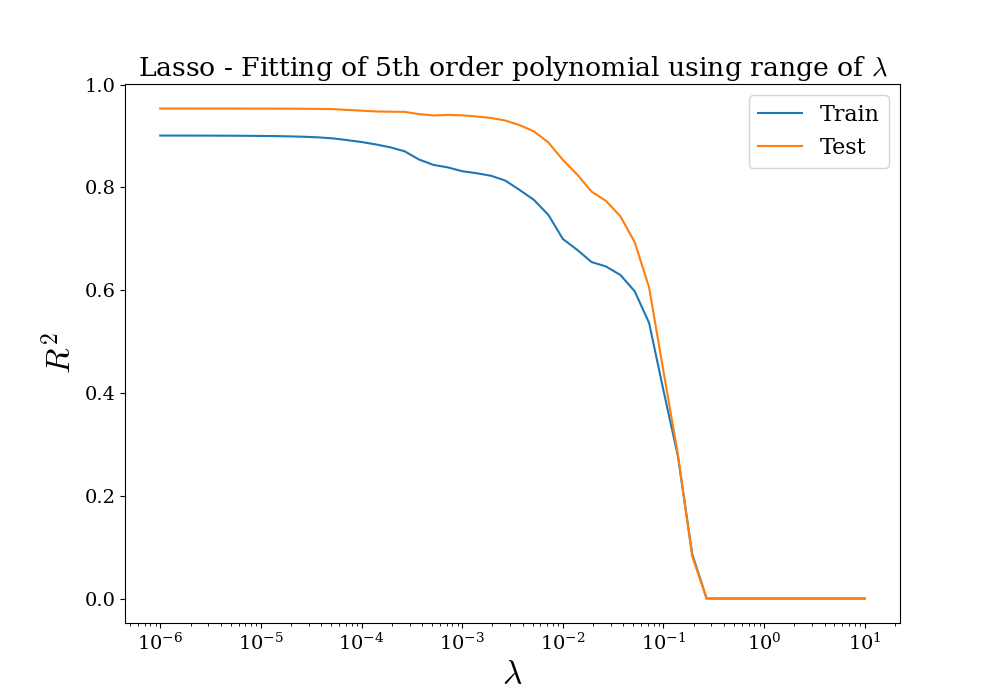
\includegraphics[width=1.0\textwidth]{../runsAndAdditions/R2OverLambdaLasso5.png}
    \end{center}
\end{minipage}\\


\begin{minipage}[!t]{.48\linewidth}
    \begin{center}
        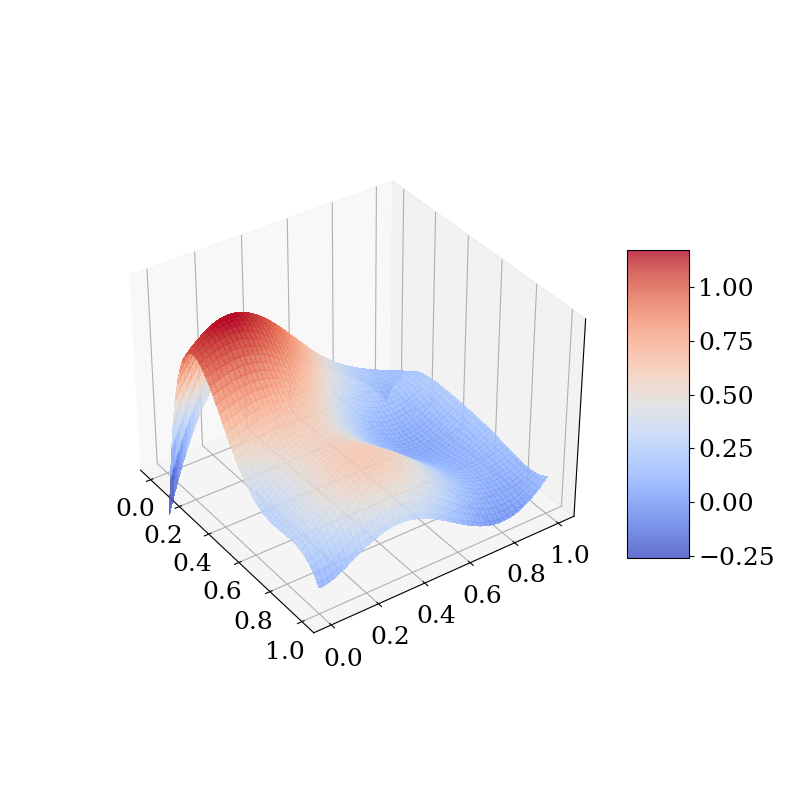
\includegraphics[width=1.0\textwidth]{../runsAndAdditions/predictionOLS.png}
\end{center}
\end{minipage}
\hspace{4mm}
\begin{minipage}[!t]{.48\linewidth}
    \begin{center}
        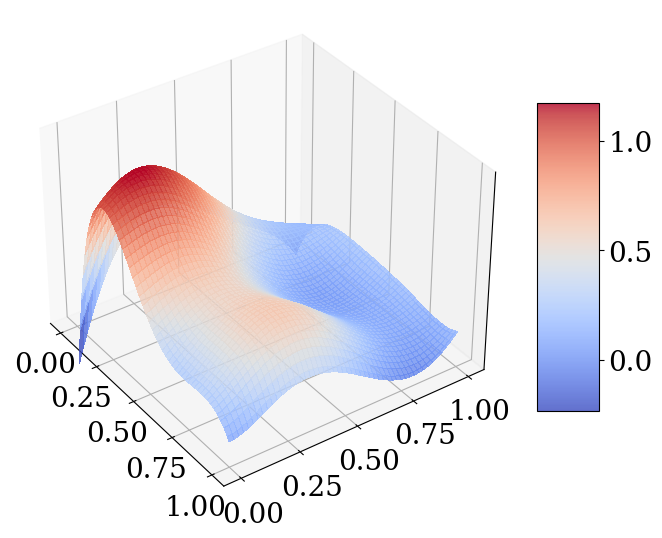
\includegraphics[width=1.0\textwidth]{../runsAndAdditions/predictionRidge.png}
    \end{center}
\end{minipage}

\begin{minipage}[!t]{.48\linewidth}
    \begin{center}
        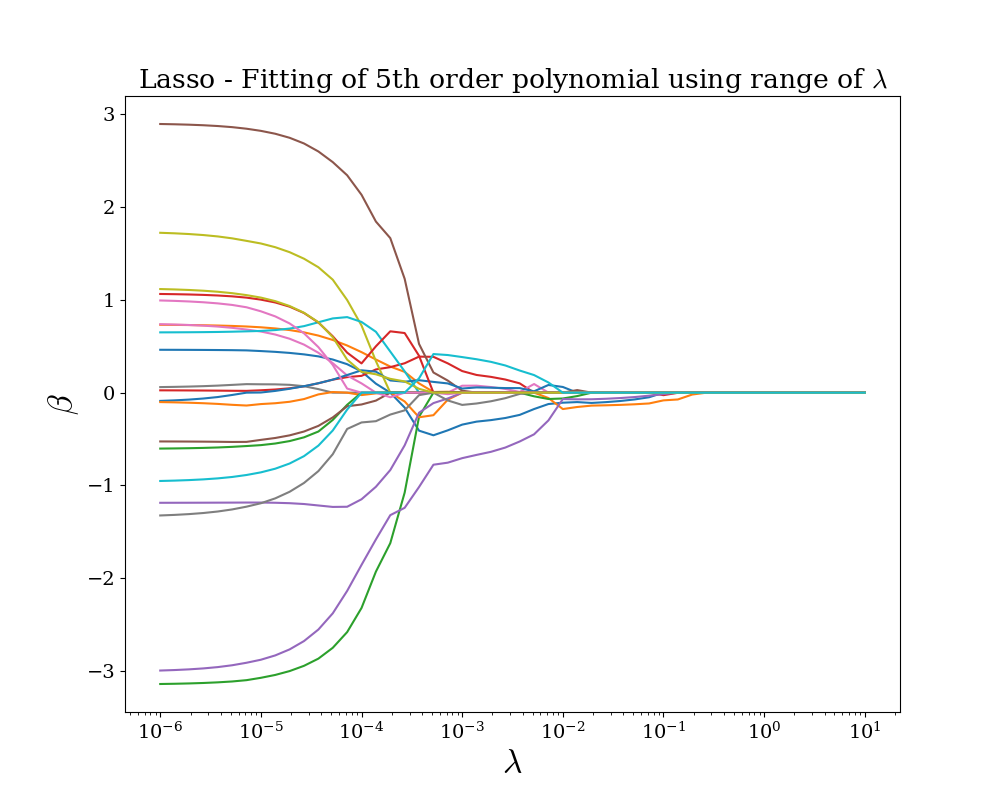
\includegraphics[width=1.0\textwidth]{../runsAndAdditions/betaOverLambdaLasso5.png}
\end{center}
\end{minipage}
\hspace{4mm}
\begin{minipage}[!t]{.48\linewidth}
    \begin{center}
        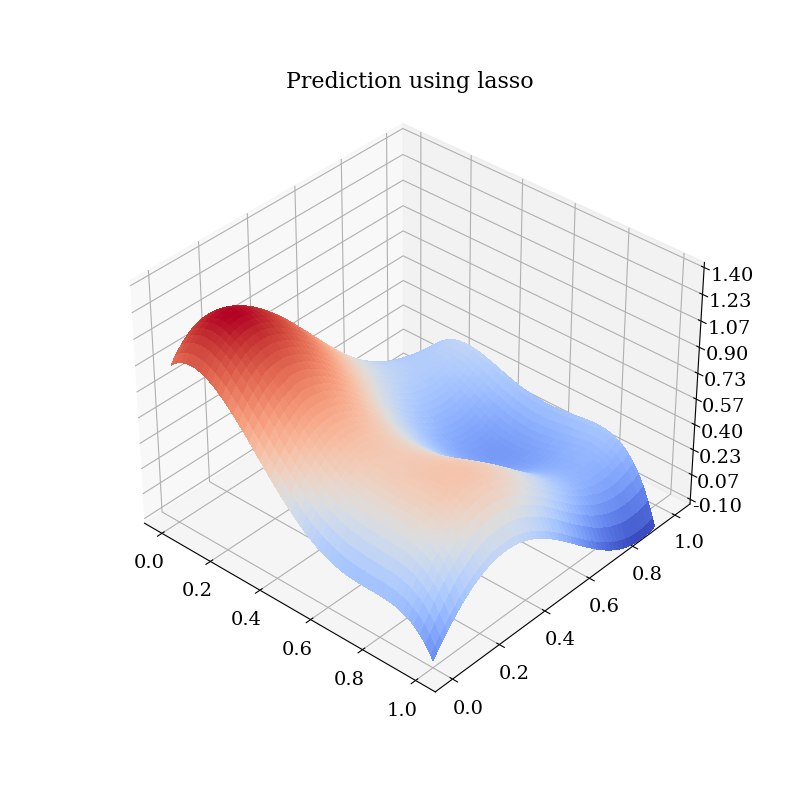
\includegraphics[width=1.0\textwidth]{../runsAndAdditions/predictionLasso.png}
    \end{center}
\end{minipage}\\

\begin{minipage}[!t]{.48\linewidth}

\end{minipage}
\hspace{4mm}
\begin{minipage}[!t]{.48\linewidth}
    \begin{center}
        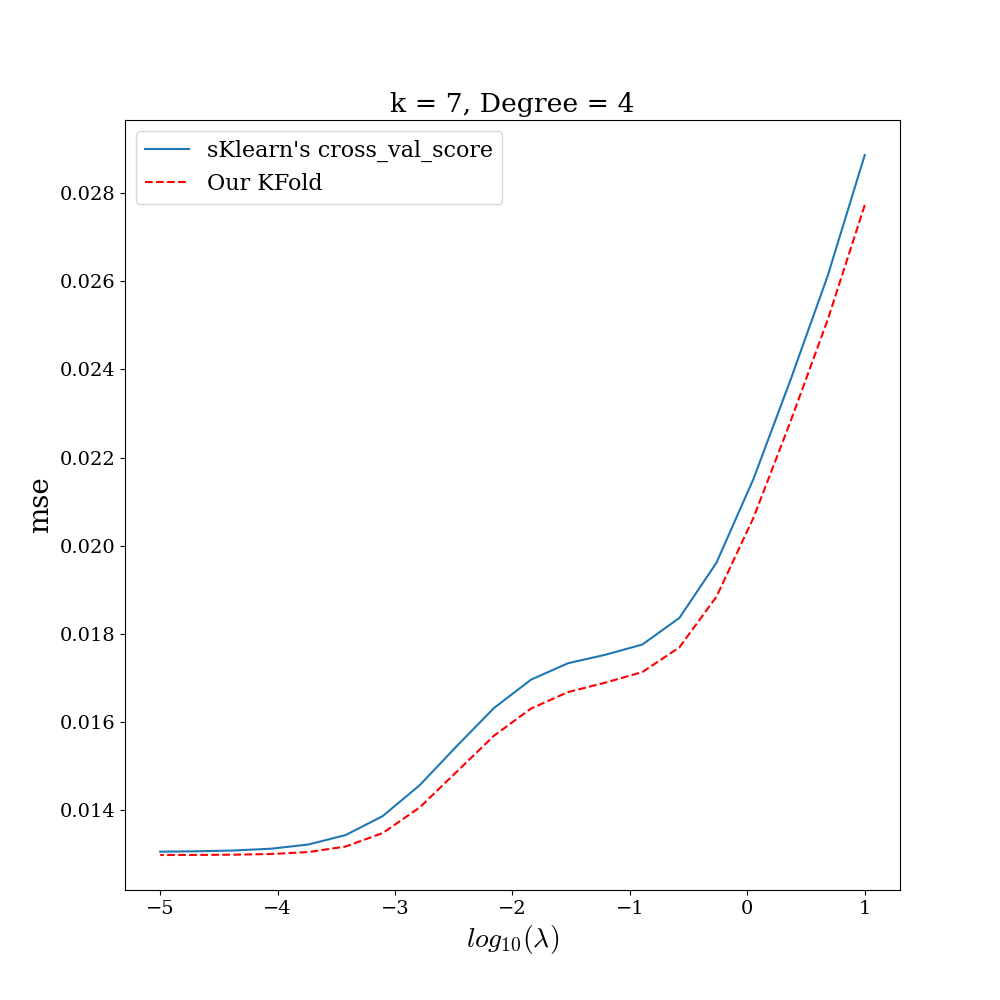
\includegraphics[width=1.0\textwidth]{../runsAndAdditions/crossvalOursVsSklearn.png}
    \end{center}
\end{minipage}\\
\begin{figure}
    \begin{center}
        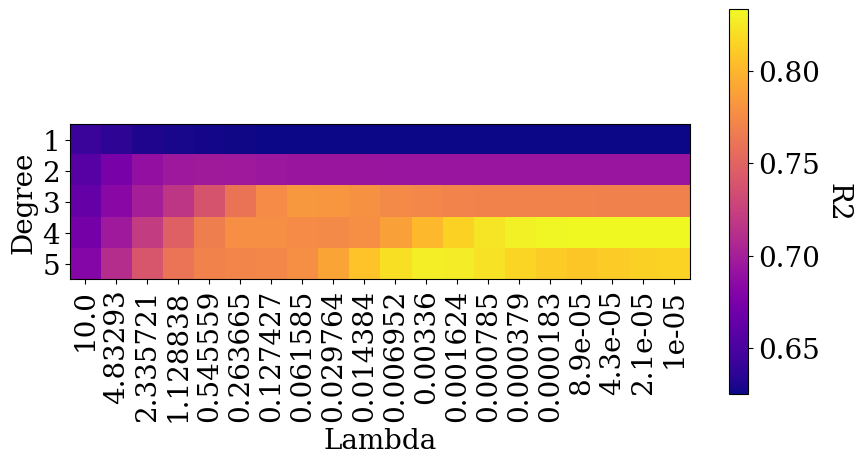
\includegraphics[width=1.0\textwidth]{../runsAndAdditions/heatmapCrossval.png}
    \end{center}
    \caption{}\label{fig:}
\end{figure}







\section{Bias \& Variance}
\label{sec:biasvariance}

It is possible to perform a so called bias-variance decomposition of our error, 
see for example Hastie et al. (2009), chapter 7.3 \cite{hastie01statisticallearning}.
By doing so we can show that the mean squared error can be written as the following

\begin{minipage}[t]{.48\linewidth}
\begin{align*}
    \text{var}(\mathbf{\tilde{y}}) &= \mathbb{E}\left[\left(\tilde{\mathbf{y}}-\mathbb{E}\left[\mathbf{\tilde{y}}\right]\right)^2\right] 
         = \mathbb{E}[\mathbf{\tilde{y}}^2] - \mathbb{E}[\mathbf{\tilde{y}}]^2\\
    \mathbb{E}[\mathbf{\tilde{y}}^2] &= \mathbb{E}[\mathbf{\tilde{y}}]^2 + \text{var}(\mathbf{\tilde{y}})
\end{align*}
\end{minipage}
\hspace{2mm}
\begin{minipage}[t]{.45\linewidth}
\begin{align*}
    \mathbb{E}[\mathbf{y\tilde{y}}] & = \mathbb{E}[\mathbf{f\tilde{y}} + \mathbf{\epsilon\tilde{y}}]\\
& = \mathbb{E}[\mathbf{f\tilde{y}}] + \mathbb{E}[\mathbf{\epsilon\tilde{y}}]\\
& = \mathbb{E}[\mathbf{f\tilde{y}}] + \mathbb{E}[\mathbf{\epsilon}]\mathbb{E}[\mathbf{\tilde{y}}]\\
& = \mathbf{f}\mathbb{E}[\mathbf{\tilde{y}}]
\end{align*}
\end{minipage}\\
\begin{align*}
\mathbb{E}[\mathbf{y}^2] & = \mathbb{E}[\mathbf{f} + \mathbf{\epsilon}]^2 = \mathbb{E}[\mathbf{f}^2 + 2\mathbf{f}\mathbf{\epsilon} + \mathbf{\epsilon}^2]\\
& = \mathbb{E}[\mathbf{f}^2] + 2\mathbb{E}[\mathbf{f}\mathbf{\epsilon}] + \mathbb{E}[\mathbf{\epsilon}^2]\\
& = \mathbb{E}[\mathbf{f}^2] + 2\mathbb{E}[\mathbf{f}]\mathbb{E}[\mathbf{\epsilon}] + \mathbb{E}[\mathbf{\epsilon}^2]\\
& = \mathbf{f}^2 + \sigma^2
\end{align*}
\begin{center}
 Bringing it all together we get 
\end{center}
\begin{align*}
\mathbb{E}\left[(\mathbf{y}-\mathbf{\tilde{y}})^2\right] & = \mathbb{E}[\mathbf{y}^2] - 2\mathbb{E}[\mathbf{y\tilde{y}}] + \mathbb{E}[\mathbf{\tilde{y}}^2]\\
& = \mathbf{f}^2 + \sigma^2 - 2\mathbf{f}\mathbb{E}[\mathbf{\tilde{y}}] + \mathbb{E}[\mathbf{\tilde{y}}^2]\\
& = \mathbf{f}^2 + \sigma^2 - 2\mathbf{f}\mathbb{E}[\mathbf{\tilde{y}}] + \mathbb{E}[\mathbf{\tilde{y}}]^2 + \text{var}(\mathbf{\tilde{y}})\\
& = (\mathbf{f} - \mathbb{E}[\mathbf{\tilde{y}}])^2 + \text{var}(\mathbf{\tilde{y}}) + \sigma^2\\
& = \text{bias}[\mathbf{\tilde{y}}]^2 + \text{var}(\mathbf{\tilde{y}}) + \sigma^2
\end{align*}


\begin{figure}[!h]
\begin{minipage}[!t]{.48\linewidth}
    \begin{center}
        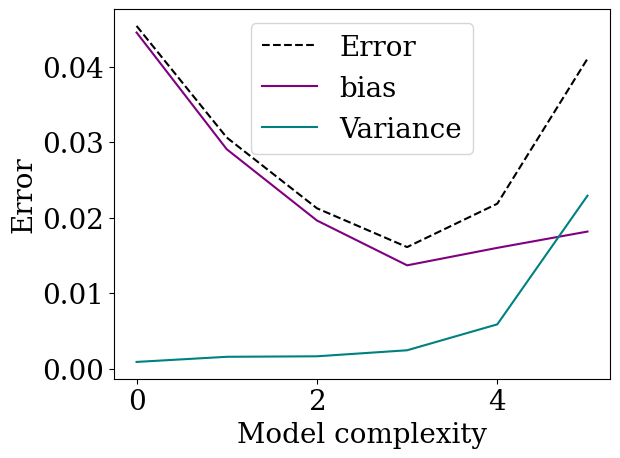
\includegraphics[width=1.0\textwidth]{../runsAndAdditions/bias-variance1.png}
        \caption{}\label{fig:bias-variance1}
    \end{center}
\end{minipage}
\hspace{2mm}
\begin{minipage}[!t]{.45\linewidth}
We need a distribution of $\mathbf{\tilde{y}}$ in order to make it possible to calculate the bias and variance of it.
We employ the bootstrap method, which generates 
multiple samples for $\mathbf{\tilde{y}}$ by using slightly different training data for each sample.
In statistical terms, \emph{variance} characterizes the spread or dispersion of our observations.
In simpler terms, a model with high variance would exhibit significant variation in the predicted values 
$\mathbf{\tilde{y}}$ from one test set to another.
If we consider Figure~\ref{fig:bias-variance2} the blue band depicts our variance, a wider band means more variance. 
The bias term measures the difference between the actual values $\mathbf{y}$ and the
expected values $\mathbf{\tilde{y}}$. This can be seen from the mathematical derivation above.
\end{minipage}
\end{figure}
It could also easily be seen from Figure~\ref{fig:bias-variance2} where the black line is the expected value of $\mathbf{\tilde{y}}$ and 
the red line is $\mathbf{y}$, notice how the closer the black line is to the red line the lower the bias is.
These two terms, bias and variance, are somewhat opposing forces. A model with high bias is likely to 
have low variance, and vice versa. As model designers, we have the flexibility to tune this trade-off. 
Depending on our priorities, whether we prioritize lower bias or lower variance, we can select an appropriate 
model to strike the right balance for our specific application.
Figure~\ref{fig:bias-variance1} and Figure~\ref{fig:bias-variance2} visualizes the classic bias-variance trade-off.
\begin{figure}[!h]
    \begin{center}
        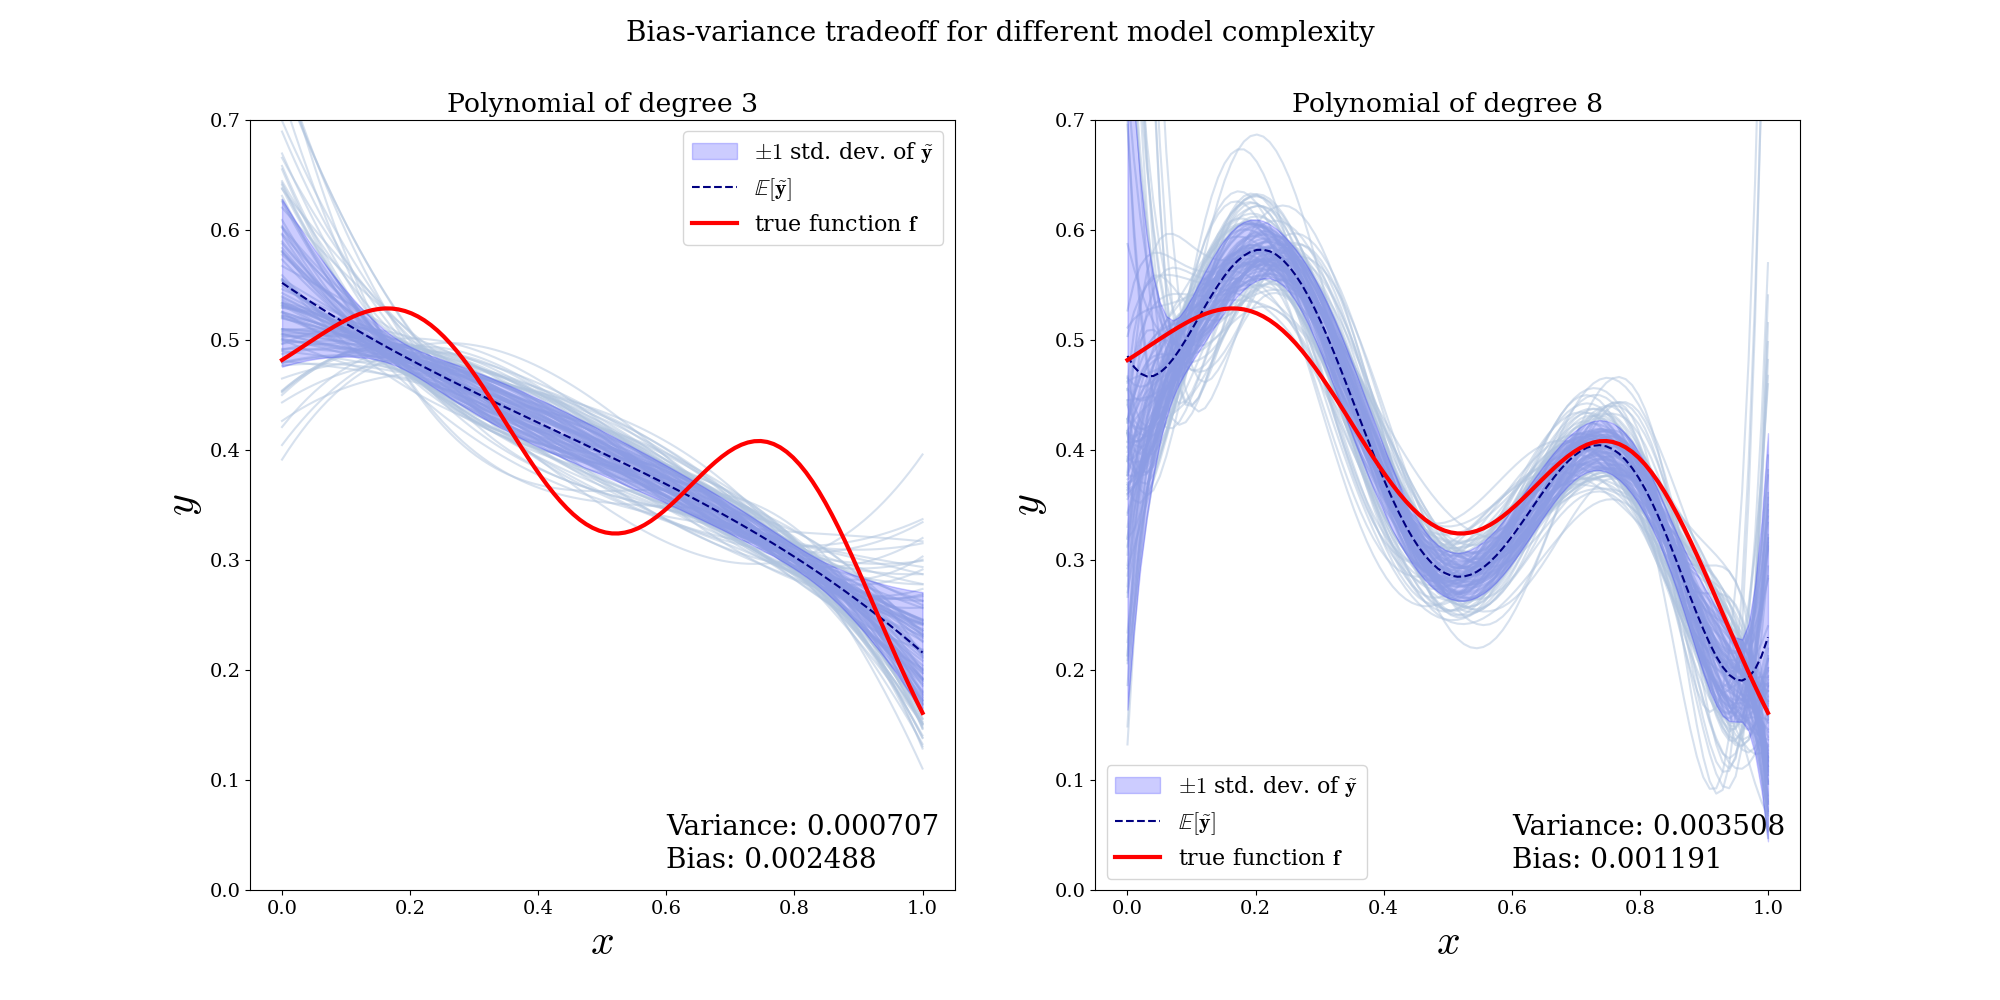
\includegraphics[width=1.0\textwidth]{../runsAndAdditions/bias-variance2.png}
    \end{center}
    \caption{Bias \& Variance Showcase, Using 2D Slice Of Our Data}\label{fig:bias-variance2}
\end{figure}








\section{Conclusion}
\label{sec:conclusion}


Lorem ipsum dolor sit amet, officia excepteur ex fugiat reprehenderit enim labore 
culpa sint ad nisi Lorem pariatur mollit ex esse exercitation amet. Nisi anim cupidatat 
excepteur officia. Reprehenderit nostrud nostrud ipsum Lorem est aliquip amet voluptate 
voluptate dolor minim nulla est proident. Nostrud officia pariatur ut officia. Sit irure 
elit esse ea nulla sunt ex occaecat reprehenderit commodo officia dolor Lorem duis laboris
cupidatat officia voluptate. Culpa proident adipisicing id nulla nisi laboris ex in Lorem 
sunt duis officia eiusmod. Aliqua reprehenderit commodo ex non excepteur duis sunt velit enim. 
Voluptate laboris sint cupidatat ullamco ut ea consectetur et est culpa et culpa duis.


















% \acks{}



% APPENDIX

%
%
\newpage
\appendix
\phantomsection%
\addcontentsline{toc}{section}{Appendix~\ref{app:appendix}}
\section*{Appendix}
\makeatletter\def\@currentlabel{A}\makeatother
\label{app:appendix}




\phantomsection%
\addcontentsline{toc}{subsection}{Derivation of The Optimal Parameters~\ref{app:OptimalBeta}}
\subsection*{Finding The Optimal Parameters $\boldsymbol{\hat{\beta}}$}
\makeatletter\def\@currentlabel{A.1}\makeatother
\label{app:OptimalBeta}

In Section~\ref{sec:ols} we ended up with our optimal parmeters $\boldsymbol{\beta}$ using the MSE as our cost function, in this section we will go into detail about our derivations.
The parameters $\boldsymbol{\beta}$ are found by minimizing our cost function (the MSE), this is done by taking the derivative of the MSE with respect to the coefficients $\beta_j$ and setting it equal to zero.

$$
{\displaystyle \min_{\boldsymbol{\beta}\in
{\mathbb{R}}^{p}}}\frac{1}{n}\sum_{i=0}^{n-1}\left(y_i-\tilde{y}_i\right)^2
$$



can also be written as 

\begin{align*}
    &{\displaystyle \min_{\mathbf{\beta}\in
{\mathbb{R}}^{p}}}\frac{1}{n}\vert\vert \mathbf{y}-\mathbf{X}\boldsymbol{\beta}\vert\vert_2^2\\
    & = \frac{2}{n}\mathbf{X}^T\left(\mathbf{X}\boldsymbol{\beta}-\mathbf{y}\right) = 0\\
    & = \frac{2}{n}\left(\mathbf{X}^T\mathbf{X}\boldsymbol{\beta}-\mathbf{X}^T\mathbf{y}\right) = 0\\
    \boldsymbol{\beta} & = \left(\mathbf{X}^T\mathbf{X}\right)^{-1}\mathbf{X}^T\mathbf{y} 
\end{align*}

$$
\hat{\boldsymbol{\beta}}_{\mathrm{OLS}} = \left(\mathbf{X}^T\mathbf{X}\right)^{-1}\mathbf{X}^T\mathbf{y},
$$
For the ridge case we have the following cost function
$$
{\displaystyle \min_{\boldsymbol{\beta}\in
{\mathbb{R}}^{p}}}\frac{1}{n}\vert\vert \mathbf{y}-\mathbf{X}\boldsymbol{\beta}\vert\vert_2^2+\lambda\vert\vert \boldsymbol{\beta}\vert\vert_2^2
$$

We know that 
$$
{\displaystyle \min_{\mathbf{\beta}\in
{\mathbb{R}}^{p}}}\frac{1}{n} \vert\vert\mathbf{y}- \mathbf{X}\boldsymbol{\beta}\vert\vert_2^2 = \frac{2}{n} \mathbf{X}^T\mathbf{X}\boldsymbol{\beta}-\frac{2}{n}\mathbf{X}^T\mathbf{y}
$$

We can also clearly see that
$${\displaystyle \min_{\mathbf{\beta}\in
{\mathbb{R}}^{p}}}\frac{1}{n} \lambda \vert\vert \mathbf{\beta}\vert\vert_2^2 = \frac{2}{n} \lambda \mathbf{\beta}
$$

Adding these two we get
\begin{align*}
   & \frac{\partial \left[\frac{1}{n}\vert\vert \mathbf{y}-\mathbf{X}\boldsymbol{\beta}\vert\vert_2^2+\lambda\vert\vert \boldsymbol{\beta}\vert\vert_2^2\right]}
    {\partial{\mathbf{\beta}}} = 0\\
                               &= \frac{2}{n}\left(\mathbf{X}^T\mathbf{X}+\lambda\mathbf{I}\right)
                               \boldsymbol{\beta}-\frac{2}{n}\mathbf{X}^T\mathbf{y} \implies \boldsymbol{\beta} = \left(\mathbf{X}^T\mathbf{X}+\lambda\mathbf{I}\right)^{-1}\mathbf{X}^T\mathbf{y}
\end{align*}



$$
\hat{\boldsymbol{\beta}}_{\mathrm{Ridge}} = \left(\mathbf{X}^T\mathbf{X}+\lambda\mathbf{I}\right)^{-1}\mathbf{X}^T\mathbf{y}
$$








\phantomsection%
\addcontentsline{toc}{subsection}{Confidence Interval~\ref{app:confidenceinterval}}
\subsection*{Confidence Interval}
\makeatletter\def\@currentlabel{A.2}\makeatother
\label{app:confidenceinterval}

We can make an assumption that there exists a continuous function $f (x)$
and a normal distributed error $\epsilon \sim n (0, \sigma^2)$ which describes our data. \footnote{This is not an assumption but rather the perfect description of our toy data. When we venture into real world data,
    we don't know if this is the case. It then becomes an assumption.}
$$ y_i = f (x_i) + \epsilon_i$$
We then approximate this function $f(x)$ with our model $\tilde{y}$ from the solution
of the linear regression equations, that is our
function $f$ is approximated by $\tilde{y}$ where we minimized $(y - \tilde{y})^2$ , with
$\tilde{y} = \mathbf{X}\boldsymbol{\beta}$
We previously derived the optimal parameters
\begin{equation}
    \label{eq:optimalbeta}
\hat{\boldsymbol{\beta}} = \left(\mathbf{X}^T\mathbf{X}\right)^{-1}\mathbf{X}^T\mathbf{y}
\end{equation}
from eq.~\ref{eq:optimalbeta} we can derive the variance of the parameters $\boldsymbol{\beta}$.
$$
\mbox{Var}(\boldsymbol{\hat{\beta}}) = \sigma^2 \, (\mathbf{X}^{T} \mathbf{X})^{-1}
$$
For ridge regression we get
$$
\mbox{Var}(\boldsymbol{\hat{\beta}}) = \sigma^2 \, (\mathbf{X}^{T} \mathbf{X} + \lambda \mathbf{I})^{-1}
$$
We also have that
$$
\mathbb{E}[\boldsymbol{\hat{\beta}}] = \boldsymbol{\beta}
$$
We can use this when we define a so-called confidence interval
for the parameters $\boldsymbol{\hat{\beta}}$. the variance of a given parameter $\beta_i$ is given by the diagonal matrix
element of the matrix $\sigma^2(\mathbf{X}^{T} \mathbf{X})^{-1}$ or $\sigma^2(\mathbf{X}^{T} \mathbf{X} + \lambda \mathbf{I})^{-1}$.
$$
z_i = \frac{\hat{\beta_i}}{\sqrt{\mbox{Var}(\hat{\beta_i})}}
$$
(Hastie et al., 2009, p. 48) \cite{hastie01statisticallearning}. 
A $z$-score of $\pm 1.96$ corresponds to a confidence interval of $95\%$

\begin{tcolorbox}
    \centering
    \textsc{ Finding the expectation value and variance of $\boldsymbol{\hat{\beta}}$}
\end{tcolorbox}

$$
\mathbb{E}(y_i)  =\sum_{j}x_{ij} \beta_j=\mathbf{X}_{i, \ast} \, \mathbf{\beta}
$$

$$
{Var}(y_i)  = \sigma^2
$$

$$
{Var}(\mathbf{\hat{\beta}}) = \sigma^2 \, (\mathbf{X}^{T} \mathbf{X})^{-1}.
$$
$$
\mathbf{y} = f(\mathbf{x}) + \epsilon
$$

$$
\mathbb{E}[\mathbf{y}] = \mathbb{E}[f(\mathbf{x} )+ \epsilon] = \mathbb{E}[f(\mathbf{x})] + \mathbb{E}[\epsilon_i]
$$

The expected value of $\epsilon_i$ is $0$, $f(x)$ is a non-stochastic variable and is approimated by $\mathbf{X}\mathbf{\beta}$

$$
\mathbb{E}[y_i] = \mathbf{X_{i,*}}\mathbf{\beta}
$$

The variance is defined as
\begin{align*}
Var(y_i) &= \mathbb{E}\big[(y_i - \mathbb{E}[y_i])^2\big] = \mathbb{E}\left[y_i^2 - 2y_i\mathbb{E}[y_i] + \mathbb{E}[y_i]^2\right] = \mathbb{E}[y_i^2] - \mathbb{E}[y_i]^2\\
Var(y_i) &= \mathbb{E}\big[\big(\mathbf{X}_{i,*}\mathbf{\beta}\big)^2 + 2\epsilon \mathbf{X}_{i,*}\mathbf{\beta} + \epsilon^2 \big] - (\mathbf{X}_{i,*}\mathbf{\beta})^2\\
Var(y_i) &= (\mathbf{X}_{i,*}\mathbf{\beta})^2 + 2\mathbb{E}[\epsilon]\mathbf{X}_{i,*}\mathbf{\beta} + \mathbb{E}[\epsilon^2] - (\mathbf{X}_{i,*}\mathbf{\beta})^2\\
Var(y_i) &= \mathbb{E}[\epsilon^2] = \sigma^2
\end{align*}
for the expected value of $\mathbf{\beta}$ we can insert the definition of $\mathbf{\beta}$ from earlier


$$
\mathbb{E}[\mathbf{\hat{\beta}}] = \mathbb{E}[ (\mathbf{X}^{\top} \mathbf{X})^{-1}\mathbf{X}^{T} \mathbf{Y}]=(\mathbf{X}^{T} \mathbf{X})^{-1}\mathbf{X}^{T} \mathbb{E}[ \mathbf{Y}]=(\mathbf{X}^{T} \mathbf{X})^{-1} \mathbf{X}^{T}\mathbf{X}\mathbf{\beta}=\mathbf{\beta}
$$


\begin{align*}
Var(\mathbf{\hat{\beta}}) & = \mathbb{E} \{ [\mathbf{\beta} - \mathbb{E}(\mathbf{\beta})] [\mathbf{\beta} - \mathbb{E}(\mathbf{\beta})]^{T} \}
\\
& = \mathbb{E} \{ [(\mathbf{X}^{T} \mathbf{X})^{-1} \, \mathbf{X}^{T} \mathbf{y} - \mathbf{\beta}] \, [(\mathbf{X}^{T} \mathbf{X})^{-1} \, \mathbf{X}^{T} \mathbf{y} - \mathbf{\beta}]^{T} \}
\\
& = (\mathbf{X}^{T} \mathbf{X})^{-1} \, \mathbf{X}^{T} \, \mathbb{E} \{ \mathbf{y} \, \mathbf{y}^{T} \} \, \mathbf{X} \, (\mathbf{X}^{T} \mathbf{X})^{-1} - \mathbf{\beta} \, \mathbf{\beta}^{T}
\\
& = (\mathbf{X}^{T} \mathbf{X})^{-1} \, \mathbf{X}^{T} \, \{ \mathbf{X} \, \mathbf{\beta} \, \mathbf{\beta}^{T} \,  \mathbf{X}^{T} + \sigma^2 \} \, \mathbf{X} \, (\mathbf{X}^{T} \mathbf{X})^{-1} - \mathbf{\beta} \, \mathbf{\beta}^{T}
\\
& = \mathbf{\beta} \, \mathbf{\beta}^{T}  + \sigma^2 \, (\mathbf{X}^{T} \mathbf{X})^{-1} - \mathbf{\beta} \, \mathbf{\beta}^{T}
\, \, \, = \, \, \, \sigma^2 \, (\mathbf{X}^{T} \mathbf{X})^{-1},
\end{align*}



ridge


$$
\mathbb{E} \big[ \hat{\mathbf{\beta}}^{\mathrm{Ridge}} \big]=(\mathbf{X}^{T} \mathbf{X} + \lambda \mathbf{I}_{pp})^{-1} (\mathbf{X}^{\top} \mathbf{X})\mathbf{\beta}.
$$


$$
{Var}[\hat{\mathbf{\beta}}^{\mathrm{Ridge}}]=\sigma^2[  \mathbf{X}^{T} \mathbf{X} + \lambda \mathbf{I} ]^{-1}  \mathbf{X}^{T}\mathbf{X} \{ [  \mathbf{X}^{\top} \mathbf{X} + \lambda \mathbf{I} ]^{-1}\}^{T},
$$


$$
\mathbb{E}[\mathbf{\hat{\beta}}^{\mathrm{Ridge}}] = \mathbb{E}\left[ \left(\mathbf{X}^T\mathbf{X}+\lambda\mathbf{I}_{pp}\right)^{-1}\mathbf{X}^T\mathbf{y}\right]=\left(\mathbf{X}^T\mathbf{X}+\lambda\mathbf{I}_{pp}\right)^{-1}\mathbf{X}^T \mathbb{E}[ \mathbf{Y}]=\left(\mathbf{X}^T\mathbf{X}+\lambda\mathbf{I}_{pp}\right)^{-1}\left(\mathbf{X}^T  \mathbf{X}\right)\mathbf{\beta}
$$

$$
\mbox{Var}(\mathbf{\hat{\beta}}^{\mathrm{Ridge}})  = \mathbb{E} \{ [\mathbf{\beta} - \mathbb{E}(\mathbf{\beta})] [\mathbf{\beta} - \mathbb{E}(\mathbf{\beta})]^{T} \}
$$
$$
\left(\mathbf{X}^T\mathbf{X}+\lambda\mathbf{I}_{pp}\right)^{-1} := \mathbf{A} 
$$
\begin{align*}
& = \mathbb{E} \left\{ \left[\mathbf{A}\mathbf{X}^T\mathbf{y} - \mathbf{A}\left(\mathbf{X}^T  \mathbf{X}\right)\mathbf{\beta}\right]
 \, 
\left[\mathbf{A}\mathbf{X}^T\mathbf{y} - \mathbf{A}\left(\mathbf{X}^T  \mathbf{X}\right)\mathbf{\beta}\right]^{T} \right\}
 \\
& = \mathbb{E} \left\{ \mathbf{A}\mathbf{X}^T \, \mathbf{y} \, \mathbf{y}^{T} \, \mathbf{X} \, \mathbf{A} - \mathbf{A}\left(\mathbf{X}^T  \mathbf{X}\right)\mathbf{\beta} \, \mathbf{\beta}^{T} \left(\mathbf{X}^T  \mathbf{X}\right) \mathbf{A} \right\}
 \\
& =  \mathbf{A}\mathbf{X}^T \, \mathbb{E} \{ \mathbf{y} \, \mathbf{y}^{T} \} \, \mathbf{X} \, \mathbf{A} - \mathbf{A}\left(\mathbf{X}^T  \mathbf{X}\right)\mathbf{\beta} \, \mathbf{\beta}^{T} \left(\mathbf{X}^T  \mathbf{X}\right) \mathbf{A}
\\
& = \mathbf{A}\mathbf{X}^T \, \left(\mathbf{X} \, \mathbf{\beta} \, \mathbf{\beta}^{T} \,  \mathbf{X}^{T} + \sigma^2 \mathbf{I}\right) \, \mathbf{X} \, \mathbf{A} - \mathbf{A}\left(\mathbf{X}^T  \mathbf{X}\right)\mathbf{\beta} \, \mathbf{\beta}^{T} \left(\mathbf{X}^T  \mathbf{X}\right) \mathbf{A}
\\
& = \boldsymbol{A}\boldsymbol{X}^T \, \left(\mathbf{X} \, \boldsymbol{\beta} \, \boldsymbol{\beta}^{T} \,  \mathbf{X}^{T} + \sigma^2 \mathbf{I}\right) \, \mathbf{X} \, \boldsymbol{A} - \boldsymbol{A}\left(\mathbf{X}^T  \mathbf{X}\right)\boldsymbol{\beta} \, \boldsymbol{\beta}^{T} \left(\mathbf{X}^T  \mathbf{X}\right) \boldsymbol{A}
\\
& = \boldsymbol{A}\boldsymbol{X}^T\boldsymbol{X}\boldsymbol{\beta}\boldsymbol{\beta}^T\boldsymbol{X}^T\boldsymbol{X}\boldsymbol{A} + \sigma^2\boldsymbol{A}\boldsymbol{X}^T\boldsymbol{X}\boldsymbol{A} - \boldsymbol{A}\boldsymbol{X}^T\boldsymbol{X}\boldsymbol{\beta}\boldsymbol{\beta}^T\boldsymbol{X}^T\boldsymbol{X}\boldsymbol{A}
\\
& = \sigma^2\boldsymbol{A}\boldsymbol{X}^T\boldsymbol{X}\boldsymbol{A} 
\\
& = \: \sigma^2[  \mathbf{X}^{T} \mathbf{X} + \lambda \mathbf{I} ]^{-1}  \mathbf{X}^{T}\mathbf{X} \{ [  \mathbf{X}^{\top} \mathbf{X} + \lambda \mathbf{I} ]^{-1}\}^{T}
\end{align*}





\vskip 0.2in
\bibliography{report}
% \bibliographystyle{apalike}
\bibliographystyle{plain}
\phantomsection%
\addcontentsline{toc}{section}{Bibliography}
\end{document}








